\section{Processament de les dades}\label{sec:data-processing}

\begin{frame}{Registres d'accés}

\begin{figure}
    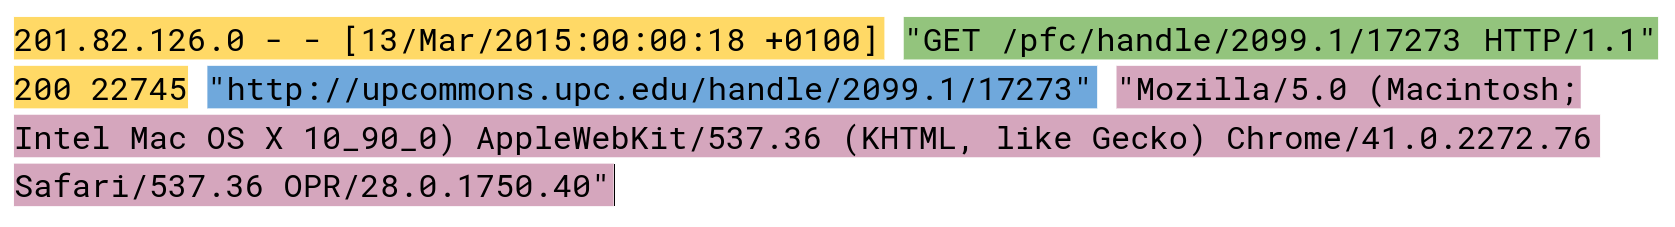
\includegraphics[width=\textwidth]{figures/example-log}
    \label{fig:log-example}
\end{figure}

\begin{itemize}%[<+- | alert@+>]
    \item Informació de la petició HTTP.
    \begin{itemize}%[<+- | alert@+>]
        \item Adreça IP: informació \textbf{personal}, s'ha hagut de passar per un procés d'anonimització.
        \item Data i hora
        \item Informació de la petició HTTP
        \item Referent
        \item User Agent
    \end{itemize}
\end{itemize}

\end{frame}

\begin{frame}{Filtratge dels \textit{logs} I}
    \begin{itemize}%[<+- | alert@+>]
        \item Durant el processament hem trobat diverses casuístiques que s'han de tractar detalladament.
        \begin{itemize}%[<+- | alert@+>]
            \item Accés a recursos web.
            \item Repeticions.
            \item Cerques.
            \item Errors de processament.
            \begin{itemize}%[<+- | alert@+>]
                \item Errors reversibles.
                \item Errors irreversibles.
            \end{itemize}
        \end{itemize}
    \end{itemize}
\end{frame}

\begin{frame}{Accés a recursos web}
    \begin{itemize}%[<+- | alert@+>]
        \item Aquests casos els descartem.
    \end{itemize}

    \begin{figure}[htbp]
        \centerline{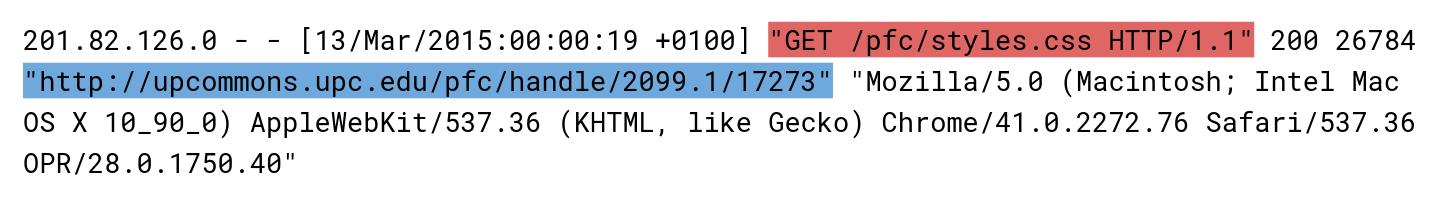
\includegraphics[width=\textwidth]{figures/log-web-resource}}
        \label{fig:log-web-resource}
    \end{figure}
\end{frame}

\begin{frame}{Repeticions}
    \begin{itemize}%[<+- | alert@+>]
        \item Accessos ``repetits'' al mateix recurs.
    \end{itemize}
    \begin{figure}[htbp]
        \centerline{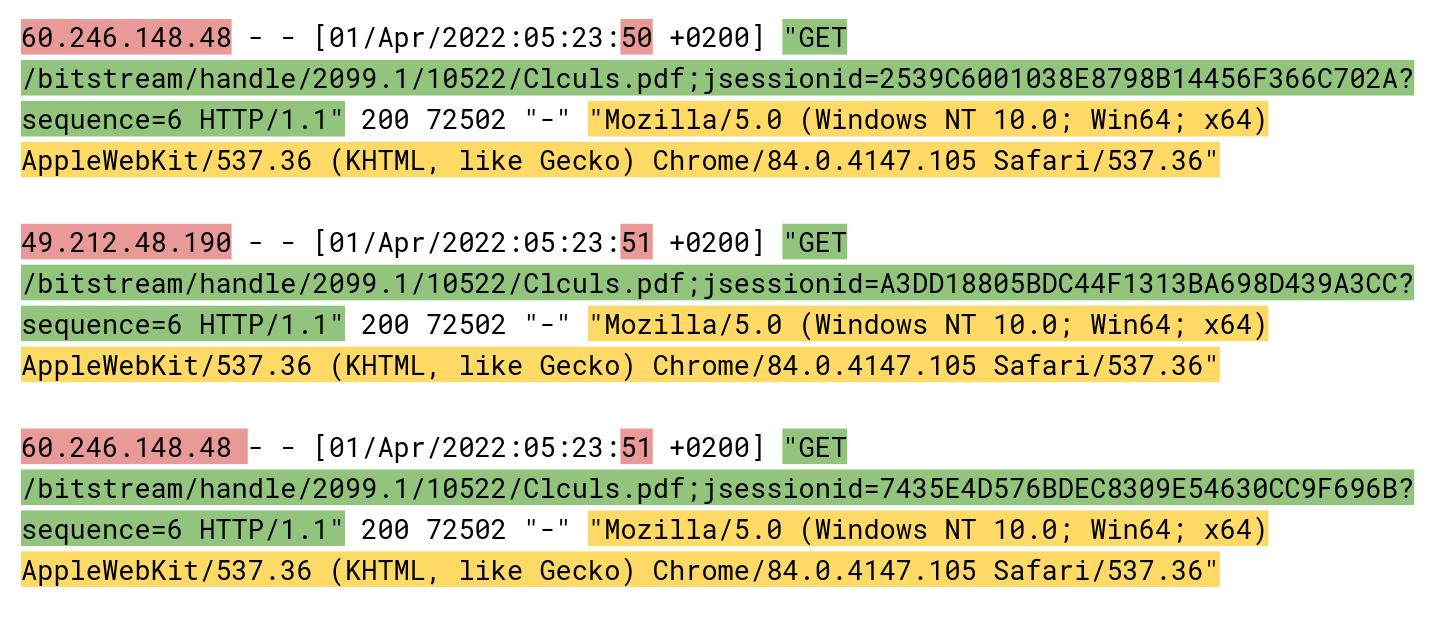
\includegraphics[width=\textwidth]{figures/log-repetitions}}
        \label{fig:log-repetitions}
    \end{figure}
\end{frame}

\begin{frame}{Cerques}
    \begin{itemize}%[<+- | alert@+>]
        \item Aquests casos els marquem com a cerques.
    \end{itemize}
    \begin{figure}[htbp]
        \centerline{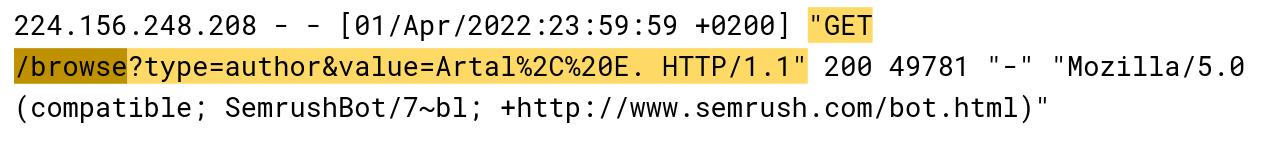
\includegraphics[width=\textwidth]{figures/log-search}}
        \label{fig:log-search}
    \end{figure}
\end{frame}

\begin{frame}{Errors de processament}
    \begin{itemize}%[<+- | alert@+>]
        \item Si l'alteració del format es menor, adaptarem el registre per homogeneïtzar el conjunt dels \textit{logs}.
        \item Els errors que no hem pogut adaptar-los s'han descartat.
    \end{itemize}
    \begin{figure}[htbp]
        \centerline{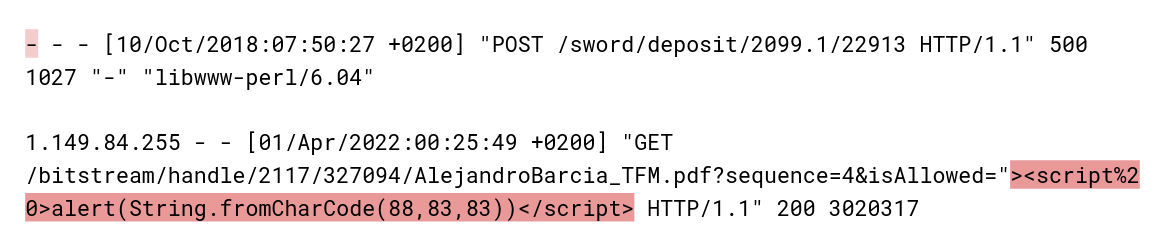
\includegraphics[width=\textwidth]{figures/log-error}}
        \label{fig:log-error}
    \end{figure}
\end{frame}

\begin{frame}{Disseny del processament dels logs}

    \begin{figure}
        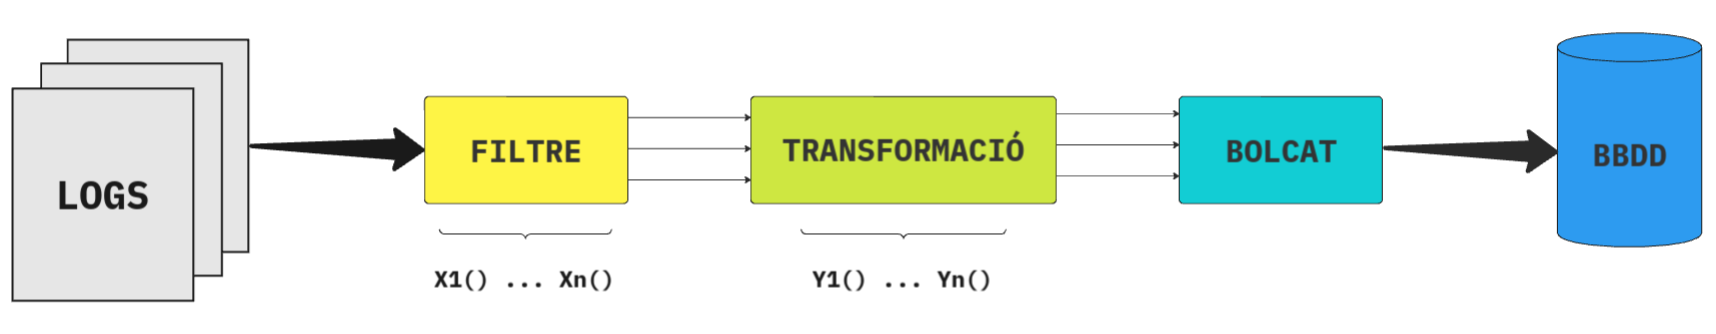
\includegraphics[width=\textwidth]{figures/log-processing}
        \label{fig:log-processing}
    \end{figure}

    \begin{itemize}%[<+- | alert@+>]
        \item Tres components.
        \begin{itemize}%[<+- | alert@+>]
            \item \texttt{Filtre} \(\rightarrow\) Filtra cada \textit{log} mitjançant un criteri específic.
            \item \texttt{Transformació} \(\rightarrow\) Modifica el format del \textit{log} per afegir o treure camps.
            \item \texttt{Bolcat} \(\rightarrow\) Adapta el format i envia el \textit{log} a la base de dades.
        \end{itemize}
    \end{itemize}
\end{frame}


\begin{frame}{Implementació del processament}
    \vfill
    \noindent
    \begin{adjustbox}{max size={1.175\textwidth}{\textheight},center}
        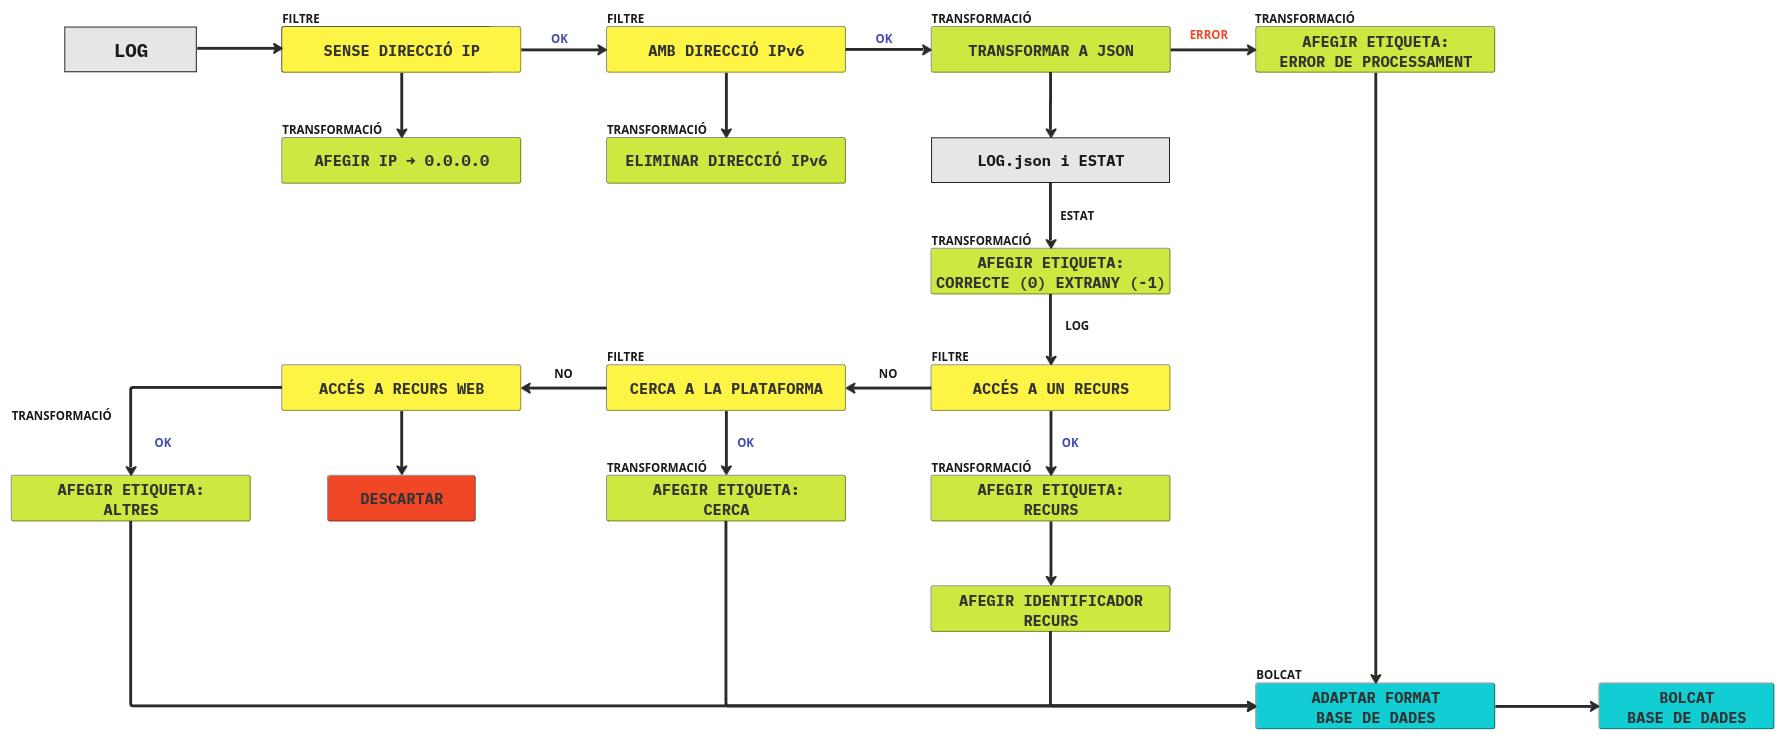
\includegraphics{figures/log-processing-workflow}
    \end{adjustbox}
    \vfill
\end{frame}


\begin{frame}{Metadades}
    \begin{itemize}%[<+- | alert@+>]
        \item Conjunt d’etiquetes presents als recursos d’UPCommons que contenen informació sobre aquest.
        \item Format: DSpace Intermediate Metadata (DIM):
        \begin{itemize}%[<+- | alert@+>]
            \item Dublin Core + qualificador.
        \end{itemize}
        \item Exemple: autor principal d'un recurs.
        \begin{itemize}%[<+- | alert@+>]
            \item \texttt{schema.element.qualifier} \(\rightarrow\) \texttt{dc.contributor.author}
        \end{itemize}
    \end{itemize}
\end{frame}


\begin{frame}{Descàrrega de les metadades}

    \begin{figure}
        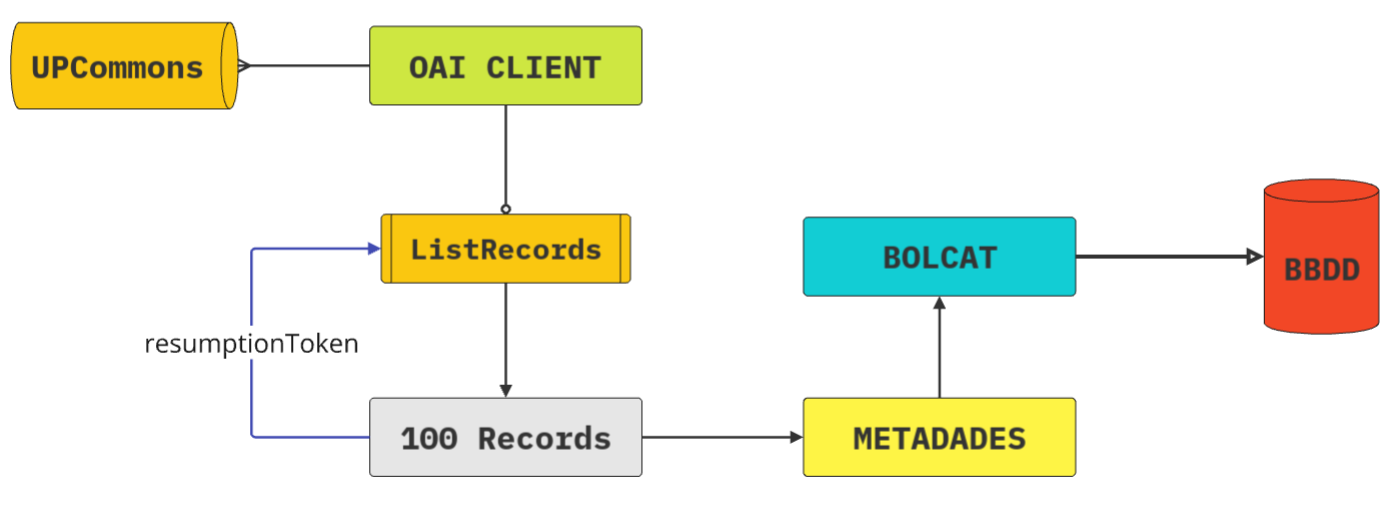
\includegraphics[width=\textwidth]{figures/metadata-processing}
        \label{fig:metadata-processing}
    \end{figure}

    \begin{itemize}%[<+- | alert@+>]
        \item Utilitzarem el protocol OAI-PMH (Open Archive Initiative-Protocol for Metadata Harvesting).
        \item El servidor que emmagtzema aquestes metadades implementa un mecansime de control de flux basat en el \textit{resumptionToken}.
    \end{itemize}

\end{frame}